\documentclass[alsotrans]{beamerswitch}
\usepackage{sdp}

\title{Речници}

\date[16.12.2019 г. -- 6.01.2020 г.]{16 декември 2019 г. -- 6 януари 2020 г.}

\titlegraphicx{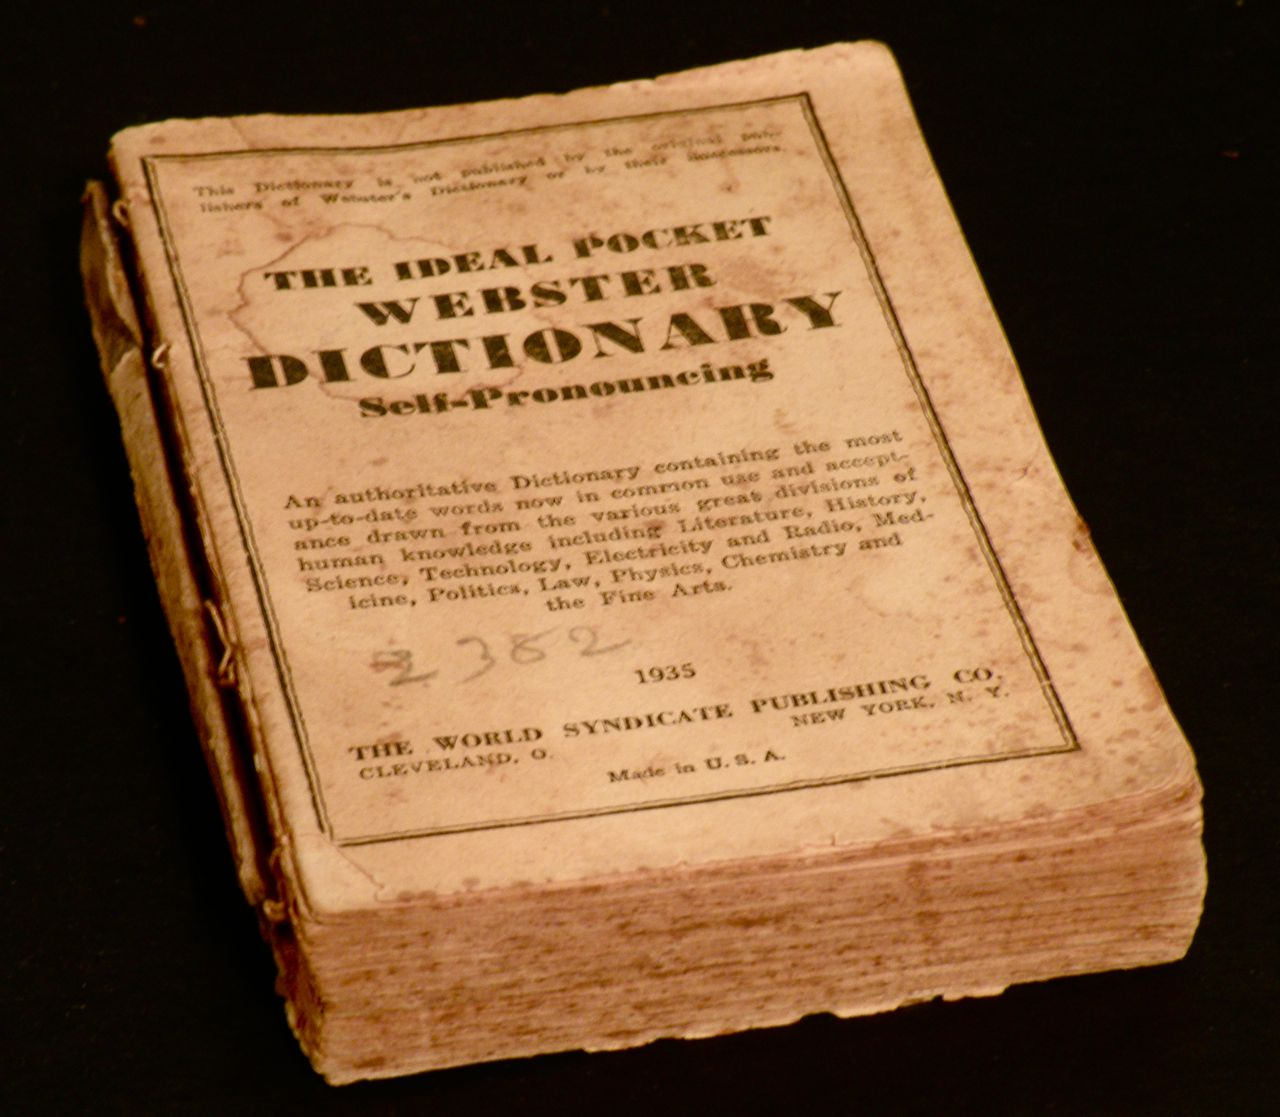
\includegraphics[height=0.25\textheight]{images/hash.jpg}\\
  \imageBased{A Dictionary Of The English Language}{Jurriaan Persyn}{https://flic.kr/p/6ThMfe}{CC BY-NC 2.0}}

\begin{document}

\begin{frame}
  \titlepage
\end{frame}

\section{АТД речник и реализации}

\begin{frame}
  \frametitle{АТД: Речник}
  Структура, представяща функционална връзка между две множества от елементи (ключове и стойности).\\[2ex]
  \pause
  Още известна като: асоциативен списък (associative list) и карта (map)\\[2ex]
  \pause
  Операции
  \begin{itemize}
  \item \tt{create()} --- създаване на празен речник
  \item \tt{lookup(key)} --- търсене на стойност по ключ
  \item \tt{add(key, value)} --- добавяне на връзка между ключ и стойност
  \item \tt{remove(key)} --- изтриване на ключ и свързаната с него стойност
  \item \tt{keys()} --- списък от всички ключове
  \item \tt{values()} --- списък от всички стойности
  \end{itemize}
\end{frame}

\begin{frame}
  \frametitle{Реализация: списък}
  Свързан списък от двойки (ключ, стойност)
  \pause
  \begin{itemize}
  \item \tt{lookup(key)} \onslide<+(1)->{--- $O(n)$, обхождането е в реда на включването}
  \item \tt{add(key, value)} \onslide<+(1)->{--- $O(1)$, винаги в края на списъка}
  \item \tt{remove(key)} \onslide<+(1)->{--- $O(n)$, първо ключът трябва да бъде намерен}
  \end{itemize}
\end{frame}

\begin{frame}
  \frametitle{Реализация: сортиран списък}
  Свързан списък от двойки (ключ, стойност), сортиран по ключове (считаме, че имаме наредба по ключовете)
  \pause
  \begin{itemize}
  \item \tt{lookup(key)} \onslide<+(1)->{--- $O(n)$, отново може да се наложи да обходим целия списък!}
  \item \tt{add(key, value)} \onslide<+(1)->{--- \alert{$O(n)$}, търсим мястото на новия ключ}
  \item \tt{remove(key)} \onslide<+(1)->{--- $O(n)$, първо ключът трябва да бъде намерен}
  \end{itemize}
\end{frame}

\begin{frame}
  \frametitle{Реализация: сортиран масив}
  Динамичен масив от двойки (ключ, стойност), сортиран по ключове\\
  \pause
  Алгоритъм за двоично търсене:
  \begin{enumerate}
  \item търсим ключ \tt Y в сортиран масив в интервала \tt{[left; right]}
  \item първоначално \tt{left = 0}, \tt{right = n - 1}
  \item\label{it:start}  намираме средата на масива \tt{mid = (left + right) / 2}
  \item сравняваме търсения ключ \tt Y с ключа \tt X на позиция mid
  \item ако \tt{Y == X} --- успех
  \item ако \tt{Y < X} --- търсим \tt Y отляво, \tt{right = mid - 1} и към \ref{it:start}
  \item ако \tt{Y > X} --- търсим \tt X отдясно, \tt{left = mid + 1} и към \ref{it:start}
  \end{enumerate}
  \pause
  \begin{itemize}
  \item \tt{lookup(key)} \onslide<+(1)->{--- $O(\log n)$, можем да използваме двоично търсене}
  \item \tt{add(key, value)} \onslide<+(1)->{--- $O(n)$, може да разместим всички елементи}
  \item \tt{remove(key)} \onslide<+(1)->{--- $O(n)$, може да разместим всички елементи}
  \end{itemize}
\end{frame}

\begin{frame}
  \frametitle{Реализация: двоично дърво за търсене}
  Двоично дърво за търсене с двойки (ключ, стойност), като се използва наредбата между ключовете
  \pause
  \begin{itemize}[<+->]
  \item обикновено двоично дърво за търсене
    \begin{itemize}
    \item \tt{lookup}, \tt{add}, \tt{remove} са със средна сложност $O(\log n)$\ldots
    \item \ldots но са с най-лоша сложност $O(n)$
    \end{itemize}
  \item самобалансиращо се дърво за търсене (AVL, червено-черно, \ldots)
    \begin{itemize}
    \item \tt{lookup}, \tt{add}, \tt{remove} са със най-лоша и средна сложност \alert{$O(\log n)$}
    \end{itemize}
  \item $B$-дърво
    \begin{itemize}
    \item същата сложност като при самобалансиращи се дървета
    \item допълнително предимство: всеки възел е с фиксиран размер
    \item<.-> може да се избере да съвпада с физически/логически сектор на външно записващо устройство
    \item<.-> това може да доведе до увеличаване на производителността
    \end{itemize}
  \end{itemize}
\end{frame}

\section{Хеш таблица}

\begin{frame}
  \frametitle{Хеш таблица}
  Масив с фиксиран размер $n$ от двойки (ключ, стойност).
  \begin{itemize}[<+->]
  \item \textbf{Основна идея:} На базата на ключ $k$ бързо да определяме индекс в масива $i_k$, където той трябва да бъде търсен, добавен или изтрит
  \item \textbf{Частен случай:} Допустимите ключове са последователните цели числа от 0 до $m < n$
  \item В този случай съпоставяме на всеки ключ индекс със същия номер $i_k := k$
  \item Какво да правим в останалите случаи?
  \item Търсим \textbf{функция} $h : Key \rightarrow [0; n)$, която да изчислява индекса съответстващ на всеки ключ, т.е. $i_k := h(k)$
  \end{itemize}
\end{frame}

\begin{frame}
  \frametitle{Хеш функции}
  Каква трябва да бъде функцията $h : Key \rightarrow [0; n)$?
  \begin{itemize}[<+->]
  \item \textbf{инекция}, ако е възможно\onslide<+->, т.е. ако $|Key| \leq n$
    \begin{itemize}
    \item  ако $|Key| > n$ със сигурност ще има $k_1 \neq k_2$, така че $h(k_1) = h(k_2)$
    \item такава ситуация нарича \textbf{колизия}
    \end{itemize}
  \item \textbf{сюрекция}, ако $|Key| > n$ за да може да се изпълни целият масив
  \item \textbf{равномерна}, т.е. с минимална вероятност за колизии
    \begin{itemize}
    \item може да се постигне, ако стойностите на $h$ (индексите) са колкото се може по-равномерно разпределени
    \item т.е. всеки индекс да се получава с приблизително равна вероятност при случаен избор на ключове
    \item т.е. всички множества $h^{-1}(i)$ са с приблизително еднаква големина
    \item тази характеристика се мери със статистически методи ($\chi^2$ тест)
    \end{itemize}
  \item функциите с горните свойства, се наричат \alert{хеш функции}
  \item стойностите $h(k)$ се наричат \alert{хеш кодове}
  \end{itemize}
\end{frame}

\begin{frame}
  \frametitle{Разрешаване на колизии}
  В практическите случаи колизиите са неизбежни и трябва да имаме стратегия за справяне с тях.\\[4ex]
  \pause
  Има две основни стратегии за разрешаване на колизии:
  \begin{itemize}
  \item разрешаване чрез пряко свързване
  \item разрешаване чрез отворено адресиране
  \end{itemize}
\end{frame}

\begin{frame}
  \frametitle{Разрешаване с пряко свързване}
  \textbf{Идея:} на всяка позиция в хеш таблицата съпоставяме ``кофа'' (bucket), която съдържа всички данни, чиито ключове имат еднакъв хеш код.\\
  \pause
  Нарича се още ``отворено хеширане'' или ``затворено адресиране''.\\
  \pause
  \textbf{Пример:} Нека $h(\text{"Sylvia"{}}) = 0$, $h(\text{"Ivan"{}}) = h(\text{"Peter"{}}) = h(\text{"Darina"{}}) = 5$, $h(\text{"Marina"{}}) = h(\text{"Andrey"{}}) = 10$.
  \begin{center}
    \small
    \begin{tikzpicture}
      \matrix (a) [mtx] { \&\&\&\&\&\&\&\&\&\&\&\&\&\&\&\&\&\\};
      \foreach \idx/\key in {1/Sylvia,6/Ivan,11/Marina} {
        \doublecell[below=3ex of a-1-\idx,nodes={inner sep=.5ex}]{\key}{\tt{\key}}
        \draw[pointer] (a-1-\idx.center) to (\key);
      }
      \foreach \old/\new in {Ivan/Peter,Peter/Darina,Marina/Andrey} {
        \doublecell[below=3ex of \old next,nodes={inner sep=.5ex}]{\new}{\tt{\new}}
        \draw[pointer] (\old next.center) to (\new);
      }
      \foreach \cell in {Sylvia,Darina,Andrey} { \nullptr{\cell next} }
    \end{tikzpicture}
  \end{center}
\end{frame}

\begin{frame}
  \frametitle{Разрешаване с отворено адресиране}
  \textbf{Идея:} използваме предварително фиксирана пермутация на индексите. При колизия изпробваме последователно индексите в реда, зададен в пермутацията.\\[2ex]
  \pause
  Нарича се още ``затворено хеширане''.\\[2ex]
  \pause
  \textbf{Пример:} Нека сме фиксирали пермутацията 1, 4, 5, 2, 6, 7, 0, 3.
  Нека $h(\text{"Ivan"{}}) = h(\text{"Peter"{}}) = 1$, $h(\text{"Darina"{}}) = 4$, $h(\text{"Sylvia"{}}) = h(\text{"Andrey"{}}) = 7$.
  \begin{center}
    \small
    \begin{tikzpicture}
      \matrix [mtx,nodes={minimum width=4em}] {
        |(s)| Sylvia \& |(i)| Ivan \& \& \& |(p)| Peter \& |(d)| Darina \& \& |(a)| Andrey\\
      };
      \draw[pointer,bend left=15] (i.north) to (p.north);
      \draw[pointer,bend left=30] (p.north) to (d.north);
      \draw[pointer,bend left=10] (a.south) to (s.south);
    \end{tikzpicture}
  \end{center}
\end{frame}

\begin{frame}
  \frametitle{Сравнение на двете стратегии}
  Пряко свързване
  \begin{itemize}[<+->]
  \item лесно за реализация
  \item при добре избрана хеш функция кофите остават малки
  \item разхищение на памет при малки данни
  \end{itemize}
  \onslide<+->
  Отворено адресиране
  \begin{itemize}[<+->]
  \item пести памет при малки данни
  \item пермутацията може да се генерира от вторична хеш функция
  \item при запълване на хеш-таблицата до около 70\% производителността на търсенето рязко пада и се налага преоразмеряване на масива и прехеширане на всички стойности
  \end{itemize}
\end{frame}

\begin{frame}
  \frametitle{Сложност на операциите на хеш таблица}
  Операцията \tt{lookup} има:
  \begin{itemize}[<+->]
  \item сложност $O(n)$ в най-лошия случай, когато много елементи попаднат в една кофа
  \item \alert{амортизирана средна сложност $O(1)$}
  \item амортизираната сложност се пресмята като се вземе предвид средния брой операции при продължително използване на хеш таблицата
  \end{itemize}
\end{frame}

\begin{frame}
  \frametitle{Разширение на хеш таблици}
  \begin{itemize}[<+->]
  \item при стратегия с отворено адресиране хеш таблицата може да се препълни
  \item при стратегия с пряко адресиране няма такава опасност, но се увеличава вероятността от колизии
  \item при приближаване на максимален капацитет е добре масивът да се преоразмери
  \item това налага промяна на хеш функцията и преизчисляване на някои или всички хеш кодове
  \item стратегии за разширение
    \begin{itemize}
    \item \textbf{пълно копиране} --- включване на всички елементи в новия масив след ново изчисляване на хеш кодовете им
    \item \textbf{инкременталлно разширение} --- елементите се прехвърлят постепенно, на всяка операция за добавяне, докато не се прехвърлят всички елементи. Докато това се случи, се търси и в старата и в новата хеш таблица
    \end{itemize}
  \end{itemize}
\end{frame}

\section{Криптография}

\begin{frame}
  \frametitle{Криптографски хеш функции}
  \begin{itemize}[<+->]
  \item в криптографията хеш функциите се използват за пресмятане на
    цифрови отпечатъци на блокове данни
  \item изискват се допълнителни свойства:
  \item \textbf{ефективност} ---  функцията да може да бъде пресмятана бързо
  \item \textbf{еднопосочност} ---  да е практически трудно възстановяването на оригиналните данни по хеш кода
    \begin{itemize}
    \item \alert{до момента не е доказано дали такива функции съществуват!}
    \end{itemize}
  \item \textbf{устойчивост към обръщане} --- да е практически трудно по даден блок данни намирането на друг блок със същия хеш код
  \item \textbf{устойчивост към колизии} --- да е практически трудно намирането на каквато и да е колизия
  \item \textbf{ефект на лавината} --- малки промени в данни да водят до големи промени в хеш кода
  \end{itemize}
\end{frame}

\begin{frame}
  \frametitle{Стандартни криптографски функции}
  \begin{itemize}[<+->]
  \item сред популярните съвременни криптографски функции са RIPEMD-160, SHA-256, Whirlpool
  \item за някои доскоро популярни функции, като MD5 и SHA-1 вече има доказателства, че не са устойчиви към колизии и не се препоръчват за използване в сценарии, където се разчита на това свойство
  \item популярни приложения:
    \begin{itemize}
    \item запазване на пароли и проверка за съвпадение без да се вижда самата парола
      \begin{itemize}
      \item речникови атаки: предварително пресметнати хеш кодове на думи
      \item предпазване от атаки: използване на ``сол'' --- не непременно тайна дума, която се добавя към паролата преди хеширане
      \end{itemize}
    \item цифрови отпечатъци (fingerprints) на документи
    \item (псевдо)-уникален идентификатор, базиран на съдържание
    \item доказателство за извършена работа (Bitcoin)
    \end{itemize}
  \end{itemize}
\end{frame}

\section{Множество}

\begin{frame}
  \frametitle{АТД: множество}
  Структура, която съдържа уникални елементи без определен ред.\\
  Операции
  \begin{itemize}
  \item \tt{create()} --- създаване на празно множество
  \item \tt{empty()} --- проверка за празнота
  \item \tt{insert(x)} --- включване на елемент
  \item \tt{remove(x)} --- изключване на елемент
  \item \tt{contains(x)} --- проверка за съдържане на елемент
  \item \tt{elements()} --- списък от всички елементи
  \end{itemize}
\end{frame}

\begin{frame}
  \frametitle{Реализация на множество}
  Структура от данни множество може да се реализира с използване на речник
  \begin{itemize}
  \item елементите са ключовете
  \item стойностите са фиктивни
  \item операциите на множеството наследяват операциите и тяхната сложност от съответната реализация на речник
  \item ако между елементите има наредба, може да се използва реализация на речник, която разчита на наредба
  \end{itemize}
\end{frame}

\section{STL реализации}

\begin{frame}
  \frametitle{\tt{std::map}}
  Реализация на речник чрез самобалансиращи се двоични дървета за търсене
  \begin{itemize}
  \item обикновено се реализират чрез червено-черни дървета
  \item дърветата съдържат \tt{std::pair<Key,Value>}
  \item елементите се пазят сортирани по ключ
  \end{itemize}
  Операции
  \begin{itemize}
  \item \tt{find(key)} --- намиране на асоциация по ключ
  \item \tt{insert(pair<...>(key,value))} --- вмъкване на асоциация
  \item \tt{erase(key)} --- изтриване на асоциация по ключ
  \item \tt{operator[key]} --- достъп до елемент с даден ключ, може да се използва и за вмъкване
  \item \tt{begin(), end()} --- итератор към асоциациите в речника, \textbf{сортирани по ключ}
  \end{itemize}
\end{frame}

\begin{frame}
  \frametitle{\tt{std::unordered\_map} (C++11)}
  Реализация на речник чрез хеш таблица
  \begin{itemize}
  \item колизиите се разрешават с пряко свързване
  \item може да се задават хеш функция и размер на таблицата
  \end{itemize}
  Операции
  \begin{itemize}
  \item \tt{find(key)} --- намиране на асоциация по ключ
  \item \tt{insert(pair<...>(key,value))} --- вмъкване на асоциация
  \item \tt{erase(key)} --- изтриване на асоциация по ключ
  \item \tt{operator[key]} --- достъп до елемент с даден ключ, може да се използва и за вмъкване
  \item \tt{begin(), end()} --- итератор към асоциациите в речника, \textbf{в неуточнен ред}
  \item \tt{rehash(n)} --- промяна на размера на хеш таблицата, при увеличаване всички елементи се хешират наново
  \end{itemize}
\end{frame}


\begin{frame}
  \frametitle{\tt{std::set}, \tt{std:unordered\_set} (C++11)}
  Реализации чрез дървета (\tt{std::set}) или хеш таблица (\tt{std:unordered\_set})\\
  Операции
  \begin{itemize}
  \item \tt{find(x)} --- намиране на итератор към елемент
  \item \tt{insert(x)} --- включване на елемент
  \item \tt{erase(x)} --- изключване на елемент
  \item \tt{begin(), end()} --- итератор към елементите в множеството, \textbf{сортирани} (при \tt{std::set}) или \textbf{без определен ред} (при \tt{std::unordered\_set})
  \end{itemize}
\end{frame}

\end{document}
